% =========================================================================
%  III. Contribution: experimental comparison
%  Numbers come from ../experiment/results/summary.json, cpu.csv and
%  demo_aliasing.csv. Figures 1 and 2 are made by paper_figures.py, the
%  others by run_experiment.py.
% =========================================================================
\section{Experimental Comparison}\label{sec:contribution}

Four oscillators were implemented in Python with NumPy. The code, data
and audio files are submitted with this paper.

% -------------------------------------------------------------------------
\subsection{Oscillators}\label{sec:oscillators}
All four use a phase $\varphi[n]$ that grows by $T = \fo/\fs$ every
sample and wraps from 1 back to 0. The naive oscillator turns it directly
into a sawtooth,
\begin{equation}
  s[n] = 2\varphi[n] - 1, \qquad
  \varphi[n] = \left(n\,\fo/\fs\right) \bmod 1 .
  \label{eq:naive}
\end{equation}
PolyBLEP computes $y[n] = s[n] - r[n]$, where the correction $r$ is
non-zero only in the samples just after and just before each jump
\cite{valimaki2007antialiasing},
\begin{equation}
  r[n] =
  \begin{cases}
    2t - t^2 - 1, & t = \varphi[n]/T, \quad \varphi[n] < T,\\
    t^2 + 2t + 1, & t = (\varphi[n]-1)/T, \quad \varphi[n] > 1-T,\\
    0,            & \text{otherwise}.
  \end{cases}
  \label{eq:polyblep}
\end{equation}
DPW-2 squares the naive sawtooth and takes the difference of neighbouring
samples \cite{valimaki2010dpw},
\begin{equation}
  y[n] = \frac{s^2[n] - s^2[n-1]}{4T},
  \label{eq:dpw}
\end{equation}
where the division by $4T$ restores the amplitude. The additive reference
sums only the harmonics below the Nyquist frequency,
\begin{equation}
  y[n] = -\frac{2}{\pi}\sum_{k=1}^{K}\frac{\sin(2\pi k\varphi[n])}{k},
  \qquad K = \left\lfloor \frac{\fs}{2\fo} \right\rfloor .
  \label{eq:additive}
\end{equation}

Fig.~\ref{fig:waveforms} shows why the naive oscillator fails. Its samples
lie exactly on the analog waveform, whose jump contains infinitely high
frequencies. PolyBLEP and DPW-2 move the samples next to the jump towards
those of the ideal additive signal.

\begin{figure}[!t]
  \centering
  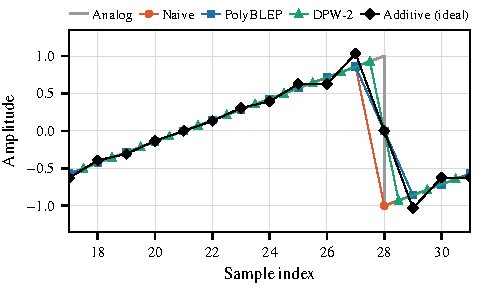
\includegraphics[width=\columnwidth]{fig_waveforms}
  \caption{Samples around one jump of a 3.15\,kHz sawtooth. DPW-2 is
  shifted by half a sample to remove its delay.}
  \label{fig:waveforms}
\end{figure}

% -------------------------------------------------------------------------
\subsection{Measuring Aliasing}\label{sec:method}
Aliasing was measured with the alias-to-harmonic ratio,
\begin{equation}
  \mathrm{AHR} = 10\log_{10}
  \frac{\sum_{f \in \mathcal{A}} |X(f)|^2}{\sum_{f \in \mathcal{H}} |X(f)|^2}
  \ \mathrm{dB},
  \label{eq:ahr}
\end{equation}
where $X(f)$ is the spectrum, $\mathcal{H}$ the frequencies within 2.7 Hz
of a harmonic and $\mathcal{A}$ all other frequencies between 20 Hz and
20 kHz. An AHR of $-30$ dB means that the aliases carry one thousandth of
the harmonic power. Fig.~\ref{fig:spectra} shows the spectra of one note,
where every line without a circle is an alias.

\begin{figure}[!t]
  \centering
  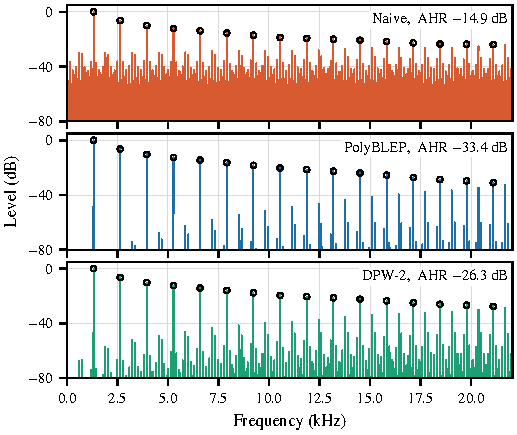
\includegraphics[width=\columnwidth]{fig_line_spectra}
  \caption{Spectra of the note E6 (1319\,Hz). Circles mark the
  harmonics.}
  \label{fig:spectra}
\end{figure}

\begin{figure}[!t]
  \centering
  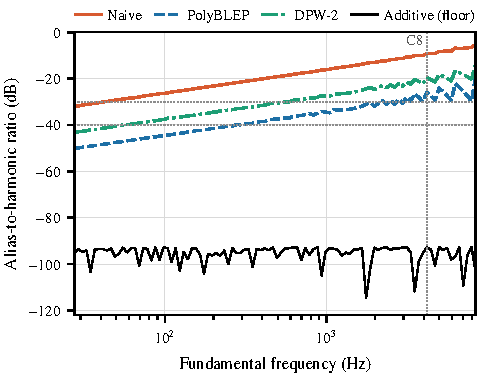
\includegraphics[width=\columnwidth]{fig_ahr}
  \caption{AHR for every note from A0 to C9. Dotted lines mark $-30$\,dB,
  $-40$\,dB and C8.}
  \label{fig:ahr}
\end{figure}

\begin{figure*}[!t]
  \centering
  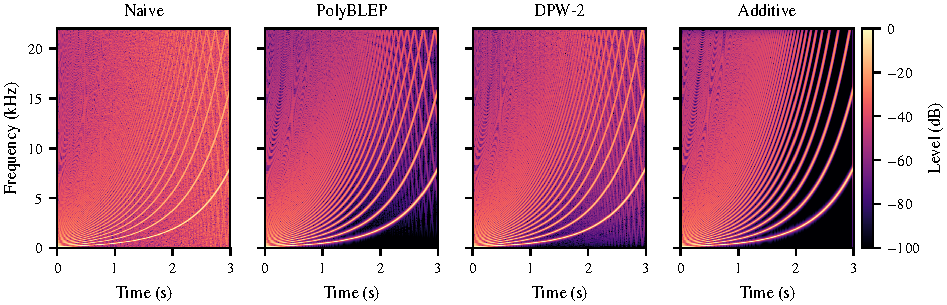
\includegraphics[width=\textwidth]{fig_spectrograms}
  \caption{Spectrograms of a 3\,s sweep from 100\,Hz to 8\,kHz. Rising
  lines are harmonics and the rest are aliases.}
  \label{fig:spectrograms}
\end{figure*}

The AHR was computed from a $2^{17}$-point FFT with a Blackman-Harris
window for all 100 notes from A0 (27.5 Hz) to C9 (8.4 kHz). For 17 notes,
such as G1, G2 and G3, the aliases land almost exactly on harmonics and
would be counted as harmonic power, so these notes were raised by up to
six cents, a few hundredths of a semitone. The AHR was also computed
with A-weighting, which weights each frequency by the sensitivity of the
ear. Finally, the harmonics of a 440 Hz tone were compared with the ideal
amplitudes $2/(\pi k)$, and computation times were measured.

% -------------------------------------------------------------------------
\subsection{Results}\label{sec:results}
Fig.~\ref{fig:ahr} and Table~\ref{tab:summary} show that the additive
oscillator stays between $-115$ and $-93$ dB, the noise floor of the
analysis. For the others, aliasing grows with pitch,
because a higher note has more of its energy above the Nyquist frequency.
The naive oscillator exceeds $-30$ dB for every note above E1 (41 Hz) and
reaches $-9$ dB at C8, the top note of the piano. PolyBLEP lowers the AHR
by 14 to 23 dB, with a median of 18 dB, and stays below $-30$ dB up to
C7 (2.1 kHz). DPW-2 lowers it by 9 to 14 dB, with a median of 11 dB, and
stays below $-30$ dB up to C\#5 (554 Hz).
A-weighting makes the corrected oscillators look better at high notes,
because their remaining aliases lie near the Nyquist frequency, where the
ear is less sensitive.

\begin{table}[!t]
  \caption{AHR in dB at Selected Notes, Highest Note Below $-30$\,dB and
  Time Relative to Naive at 440\,Hz}
  \label{tab:summary}
  \centering
  \setlength{\tabcolsep}{4pt}
  \begin{tabular}{lrrrrcr}
    \toprule
    Method & A2 & A4 & A6 & C8 & Limit & Time \\
    \midrule
    Naive    & $-25.8$ & $-19.7$ & $-13.4$ & $-9.3$  & E1   & 1.00 \\
    PolyBLEP & $-44.1$ & $-37.8$ & $-31.1$ & $-25.8$ & C7   & 1.32 \\
    DPW-2    & $-37.0$ & $-30.9$ & $-24.4$ & $-19.6$ & C\#5 & 1.45 \\
    Additive & $<-92$  & $<-92$  & $<-92$  & $<-92$  & all  & 14.4 \\
    \bottomrule
  \end{tabular}
\end{table}

The spectrograms of a rising sweep in Fig.~\ref{fig:spectrograms} show the
same order. The naive sweep is covered with aliases from
the start, PolyBLEP leaves only weak ones, and DPW-2 lies in between.

Both corrections also make the wanted high harmonics slightly quieter
(Fig.~\ref{fig:harmonics}). For a 440 Hz tone, PolyBLEP lowers the
harmonic at 19.8 kHz by 6.2 dB and DPW-2 by 3.1 dB, so DPW-2 keeps more
brightness but aliases more.

\begin{figure}[!t]
  \centering
  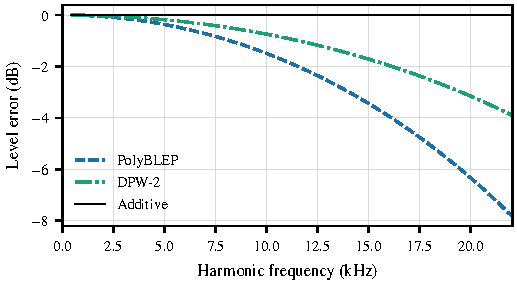
\includegraphics[width=\columnwidth]{fig_harmonics}
  \caption{Level error of the harmonics of a 440\,Hz tone.}
  \label{fig:harmonics}
\end{figure}

At 110, 440 and 1760 Hz, PolyBLEP and DPW-2 take 1.29 to 1.45 times as
long as the naive oscillator. Additive synthesis is 52 times slower at
110 Hz and 4.7 times at 1760 Hz, because lower notes need more sine
waves. These NumPy timings show relative cost only.

Two short clips show what this means in music (Table~\ref{tab:demos}).
Each was rendered with all four oscillators. In a bright lead melody
between E5 and C7 with vibrato, the aliases of the naive oscillator are
only 15 dB below the music, and PolyBLEP lowers them to $-33$ dB. In a
bass line around A1 played through a lowpass filter, the filter removes
the high aliases of PolyBLEP, which reaches $-73$ dB. The naive oscillator
also aliases far below the cutoff, so it only reaches $-33$ dB, close to
the $-29$ dB of an unfiltered A1. A filter therefore cannot replace an
antialiasing oscillator.

\begin{table}[!t]
  \caption{Aliasing in the Musical Examples in dB}
  \label{tab:demos}
  \centering
  \begin{tabular}{lrrr}
    \toprule
    Clip & Naive & PolyBLEP & DPW-2 \\
    \midrule
    Lead melody & $-15.0$ & $-33.3$ & $-26.4$ \\
    Bass line   & $-32.6$ & $-72.6$ & $-51.1$ \\
    \bottomrule
  \end{tabular}
\end{table}

% -------------------------------------------------------------------------
\subsection{Limitations}\label{sec:discussion}
The AHR ignores masking, the effect that a loud sound hides quieter sounds
nearby, so the thresholds are illustrations rather than
limits of audibility. Only DPW-2 was tested, although higher orders
perform better \cite{valimaki2010dpw}, and no formal listening test was
carried out.
